The purpose of this layer is to control the Turning Board. This layer is directly accessible to the user and takes the form of an Android and iOS apps. This layer communicates with the Main Control layer adequately to propagate user commands.

\subsection{Front-end UI and Main Control Communication }
The Front-end UI and the Main Control Layer, currently, communicate via internet. With a Firebase back-end set up, the UI interfaces with the back-end, which in turn propagates data to the Main Control. The back-end system uses a real-time NoSQL database. The Main Control, in turn, retrieves the appropriate data and passes it on to the corresponding subsystem.

\begin{figure}[h!]
	\centering
 	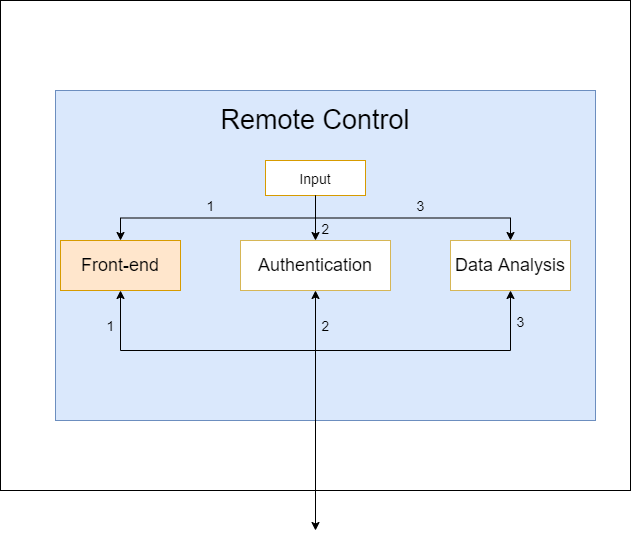
\includegraphics[width=0.60\textwidth]{ADS Latex/images/UIJetsonCom.png}
 \caption{Front-end subsystem in Remote Control Layer}
\end{figure}

\subsubsection{Assumptions}
It is assumed that the latency between data posting by the front-end and data retrieval by the Main Control is almost negligible. It is also assumed the user is always connected to the internet while the Turing Board is active.

\subsubsection{Responsibilities}
The UI must present the user with an easy to user interface. The UI must post the component's data to the real-time database as soon as the state of a component changes.

\subsubsection{Subsystem Interfaces}
Each of the inputs and outputs for the subsystem are defined here.
\begin {table}[H]
\caption {Front-end interfaces} 
\begin{center}
    \begin{tabular}{ | p{1cm} | p{6cm} | p{3cm} | p{3cm} |}
    \hline
    ID & Description & Inputs & Outputs \\ \hline
    \#1 & Giving the UI a command & \pbox{3cm}{User command} & \pbox{3cm}{\phantom{Boo!}\\raw data to a database \phantom{Boo!}\\}  \\  \hline
    \end{tabular}
\end{center}
\end{table}

\subsection{Authentication}
When the user attempts to log into the app or sign up, the UI parses the login or sign up information (i.e.name, email, password, etc.). The parsed data is then sent to a Firebase Authentication API. The API in turn forwards a token to the app confirming status of the attempt - either a successful or unsuccessful login or sign up. The app then uses the data to render the UI accordingly.

\begin{figure}[h!]
	\centering
 	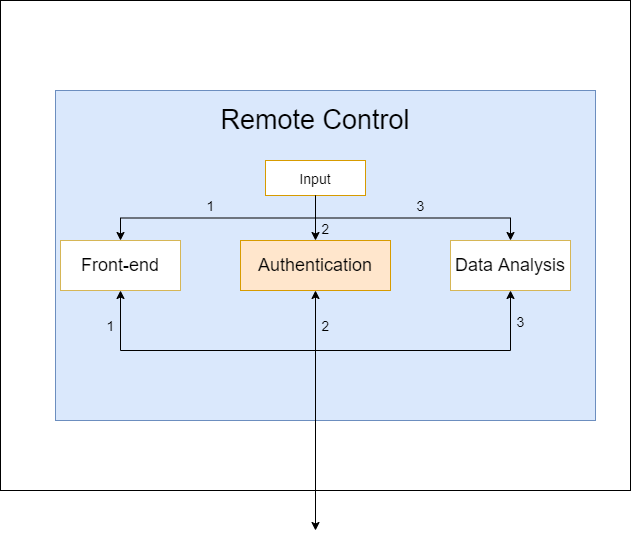
\includegraphics[width=0.60\textwidth]{ADS Latex/images/Authentication}
 \caption{Authentication subsystem in Remote Control Layer}
\end{figure}

\subsubsection{Responsibilities}
This feature determines if a user has access to the UI controller or not. It makes sure the right data will be sent to the right Turing Board.

\subsubsection{Authentication Interfaces}
Each of the inputs and outputs for the subsystem are defined here.
\begin {table}[H]
\caption {Authentication interfaces} 
\begin{center}
    \begin{tabular}{ | p{1cm} | p{6cm} | p{3cm} | p{3cm} |}
    \hline
    ID & Description & Inputs & Outputs \\ \hline
   \#2 & Authentication & \pbox{3cm}{User information} & \pbox{3cm}{Token}  \\ \hline
    \end{tabular}
\end{center}
\end{table}

\subsection{Ride Data Analysis}
This will be information provided to the user after a ride. This information may include average speed of the ride, the duration of the ride, and the distance traveled.

\begin{figure}[h!]
	\centering
 	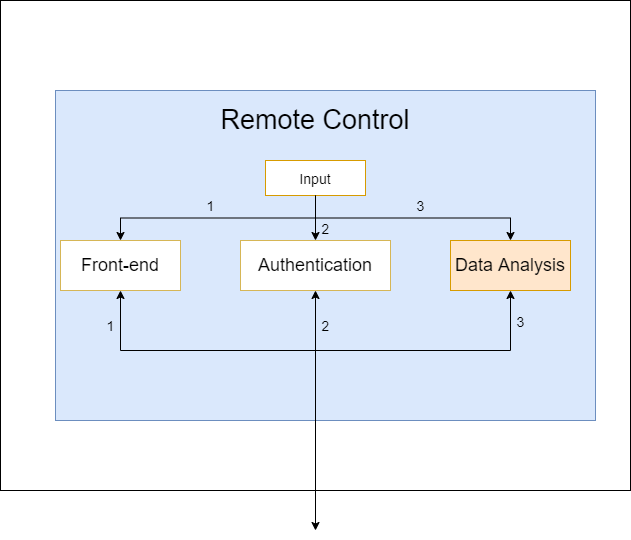
\includegraphics[width=0.60\textwidth]{ADS Latex/images/dataAnalysis.png}
 \caption{Ride Data Analysis subsystem in Remote Control Layer}
\end{figure}

\subsubsection{Responsibilities}
Provide users with their ride analysis in an understandable format.

\subsubsection{Subsystem Interfaces}
Each of the inputs and outputs for the subsystem are defined here.
\begin {table}[H]
\caption {Ride data analysis interfaces} 
\begin{center}
    \begin{tabular}{ | p{1cm} | p{6cm} | p{3cm} | p{3cm} |}
    \hline
    ID & Description & Inputs & Outputs \\ \hline
    \#3 & Ride analysis & \pbox{3cm}{\phantom{Boo!}\\refined database data\phantom{Boo!}\\} & \pbox{3cm}{legible ride analysis data}  \\ \hline
    \end{tabular}
\end{center}
\end{table}


